\documentclass[11pt,a4paper]{article}

\usepackage[utf8]{inputenc}
\usepackage[T1]{fontenc}
% NOTE : le paquet babel[french] (fichier french.ldf) n'est pas installé dans
% cet environnement et l'énoncé du TP demande de ne rien installer de plus.
% On renomme donc manuellement les libellés générés automatiquement par LaTeX
% (table des matières, figures, tableaux) pour conserver un document en
% français, sans dépendre du paquet linguistique manquant.
\usepackage[margin=2.5cm]{geometry}
\usepackage{graphicx}
\usepackage{listings}
\usepackage{xcolor}
\usepackage{booktabs}
\usepackage{array}
\usepackage{hyperref}
\usepackage{amsmath}
\usepackage{float}
\usepackage{enumitem}
\usepackage{fancyhdr}
\usepackage{titlesec}

\hypersetup{colorlinks=true, linkcolor=blue, urlcolor=blue, citecolor=blue}

\definecolor{codebg}{RGB}{245,245,245}
\definecolor{codegreen}{RGB}{0,110,0}
\definecolor{codegray}{RGB}{110,110,110}
\definecolor{codepurple}{RGB}{100,40,140}

\lstdefinestyle{python}{
    backgroundcolor=\color{codebg},
    commentstyle=\color{codegray}\itshape,
    keywordstyle=\color{codepurple}\bfseries,
    stringstyle=\color{codegreen},
    basicstyle=\ttfamily\small,
    breaklines=true,
    frame=single,
    numbers=left,
    numberstyle=\tiny\color{codegray},
    showstringspaces=false,
    tabsize=4,
    language=Python
}
\lstset{style=python}

% Renommage manuel des libellés en français (palliatif à l'absence de babel[french])
\renewcommand{\contentsname}{Table des matières}
\renewcommand{\figurename}{Figure}
\renewcommand{\tablename}{Tableau}

\pagestyle{fancy}
\fancyhf{}
\rhead{INF232 -- TP Groupe 20}
\lhead{Analyse des notes et de l'assiduité}
\cfoot{\thepage}

\title{\textbf{Rapport de Travaux Pratiques\\Analyse des notes et de l'assiduité des élèves de terminale}}
\author{Groupe 20 -- INF232\\Université de Yaoundé I}
\date{5 juillet 2026}

\begin{document}

\maketitle
\thispagestyle{empty}

\begin{center}
\begin{tabular}{|l|l|}
\hline
\textbf{Nom} & \textbf{Matricule} \\
\hline
Atangana Abogo Emmanuel (chef de groupe) & 23V2348 \\
Samaki Nya Zenouba Rhyade & 24G2773 \\
Tchatchouang Tankio Grâce Farelle & 24F2749 \\
Tsiadze Donfack Darlene & 24G2361 \\
Bissemou Francky Dilane & 24F2628 \\
Minkam Tedonfoue Kelly Dolviane & 24G2883 \\
Tchuitcheu Wouatchui Flores Backer & 24F2779 \\
Yatié Wantem Wendy Elvira & 23U2749 \\
\hline
\end{tabular}
\end{center}

\vspace{0.5cm}
\noindent\textbf{Note de correction :} la première version de ce rapport contenait une
erreur sur l'orthographe du nom du chef de groupe (« Atangana abog Emmanue » au lieu de
« Atangana Abogo Emmanuel »), utilisée pour calculer la graine de génération des données.
Cette erreur a été corrigée dans \texttt{main.py} et dans tous les scripts : la graine
correcte, calculée à partir du nom exact \texttt{ATANGANA ABOGO EMMANUEL}, vaut
\textbf{1292}. L'intégralité des résultats de ce rapport (statistiques, figures, modèles)
a été recalculée avec cette graine corrigée.

\newpage
\tableofcontents
\newpage

% ============================================================
\section{Introduction et contexte}
% ============================================================

La direction d'un établissement scolaire secondaire souhaite mieux comprendre les
performances et les profils de ses élèves de terminale à partir des résultats d'une
évaluation interne. Elle pose quatre questions concrètes, formulées dans un langage non
statistique, auxquelles ce TP répond par des méthodes issues du cours d'INF232
(statistique descriptive, corrélation, régression, apprentissage supervisé et non
supervisé).

\subsection{Variables retenues}

\begin{table}[H]
\centering
\begin{tabular}{|l|l|p{7cm}|}
\hline
\textbf{Variable} & \textbf{Symbole} & \textbf{Justification} \\
\hline
Note d'évaluation & \texttt{Notes} (X) & Mesure directe de la performance en mathématiques, sur 20 \\
Taux de présence & \texttt{Assiduité} (Y) & Indicateur de régularité et de travail personnel, en \% \\
Orientation & \texttt{target} & Décision déjà prise par le conseil de classe (0 = littéraire, 1 = scientifique) \\
\hline
\end{tabular}
\caption{Variables du jeu de données synthétique}
\end{table}

La relation imposée à la génération ($Y \approx 5X$) reflète une intuition pédagogique
raisonnable : un élève assidu tend à obtenir une meilleure note. Un bruit gaussien est
ajouté pour éviter une corrélation parfaite et produire des profils atypiques réalistes.

\subsection{Génération reproductible des données}

La reproductibilité est assurée par une graine dérivée du nom du chef de groupe, via un
hachage SHA-256 :

\begin{lstlisting}
def nettoyer_texte(texte: str) -> str:
    """Normalise : suppression des accents, majuscules."""
    texte = texte.strip()
    sans_accents = unicodedata.normalize("NFKD", texte)
    sans_accents = "".join(c for c in sans_accents
                            if not unicodedata.combining(c))
    return sans_accents.upper()  # espaces conserves

def generer_graine(texte: str) -> int:
    texte_normalise = nettoyer_texte(texte)
    hash_hex = hashlib.sha256(texte_normalise.encode()).hexdigest()
    return int(hash_hex, 16) % (2 ** 12)
\end{lstlisting}

Avec le nom correct \texttt{"Atangana Abogo Emmanuel"}, la graine obtenue est
\textbf{1292} (contre 14 avec l'ancienne orthographe erronée -- deux graines totalement
différentes, ce qui confirme qu'il fallait régénérer l'ensemble des résultats).

\begin{lstlisting}
X = rng.uniform(0, 20, 1000)              # Notes, arrondies a 0.1
bruit = rng.normal(0, 5, 1000)
Y = np.clip(5 * X + bruit, 0, 100)         # Assiduite
target = (Y >= 50).astype(int)             # 1 = scientifique
\end{lstlisting}

\begin{table}[H]
\centering
\begin{tabular}{|l|r|}
\hline
Nombre d'élèves & 1000 \\
Orientation scientifique (1) & 497 (49,7\%) \\
Orientation littéraire (0) & 503 (50,3\%) \\
\hline
\end{tabular}
\caption{Jeu de données régénéré (\texttt{data/raw/donnees.csv})}
\end{table}

\textbf{Règle du projet :} le fichier \texttt{data/raw/donnees.csv} n'est jamais modifié
après sa génération ; toutes les transformations produisent des fichiers dans
\texttt{data/interim/} ou \texttt{data/processed/}.

% ============================================================
\section{Structure du projet}
% ============================================================

Le projet suit une architecture modulaire classique en science des données,
séparant strictement code, données et résultats :

\begin{lstlisting}[language=bash]
INF232_TP_GROUPE20/
|-- data/
|   |-- raw/          # Donnees brutes generees (jamais modifiees)
|   |-- interim/       # Resultats intermediaires (stats, CSV)
|   +-- processed/     # Donnees finales pretes pour modelisation
|-- notebooks/         # Explorations interactives (Jupyter)
|-- src/
|   |-- utils/         # Graine SHA-256
|   |-- data/          # Generation et chargement
|   |-- features/      # Standardisation
|   +-- models/        # Un script par question
|-- reports/
|   +-- figures/        # Graphiques pour le rapport
+-- main.py             # Orchestration de bout en bout
\end{lstlisting}

\textbf{Justification de cette organisation :}
\begin{itemize}
\item \textbf{Séparation données/code} : \texttt{data/raw} n'est jamais écrasé, ce qui
garantit qu'on peut toujours revenir au jeu de données d'origine et vérifier la
reproductibilité (même graine $\Rightarrow$ mêmes données).
\item \textbf{Un script = une question} : chaque question du proviseur correspond à un
fichier autonome dans \texttt{src/models/}, ce qui facilite la relecture, le test et la
correction indépendante de chaque partie.
\item \textbf{\texttt{data/interim} vs \texttt{data/processed}} : distingue les résultats
de calcul intermédiaires (statistiques, matrices de corrélation) des données réellement
transformées et prêtes pour un modèle (ex. : jeu enrichi avec les clusters).
\item \textbf{\texttt{main.py}} centralise l'orchestration pour garantir que
\texttt{python main.py} rejoue l'intégralité de l'analyse dans le bon ordre
(génération $\rightarrow$ Q1 $\rightarrow$ Q2 $\rightarrow$ Q3 $\rightarrow$ Q4), condition
indispensable de reproductibilité exigée par le sujet.
\end{itemize}

% ============================================================
\section{Question 1 -- Répartition des notes}
% ============================================================

\subsection{Question posée}
\textit{« Comment se répartissent les résultats de mes élèves ? Y a-t-il des élèves dont
le résultat sort vraiment de l'ordinaire ? Comment présenter cela simplement au conseil
pédagogique, qui n'est pas formé en statistique ? »}

\subsection{Notions du cours mobilisées et méthode}

Il s'agit d'une \textbf{analyse statistique univariée} : une seule variable est étudiée
(\texttt{Notes}), sans tenir compte des autres. On utilise :
\begin{itemize}
\item les \textbf{statistiques descriptives} (moyenne, écart-type, quartiles) pour
résumer la distribution ;
\item la \textbf{règle de Tukey} pour détecter les valeurs atypiques (outliers), car elle
est robuste, simple à expliquer et ne suppose pas que les données suivent une loi
particulière (contrairement à une règle basée sur l'écart-type, plus sensible aux
valeurs extrêmes qu'elle est censée détecter).
\end{itemize}

\begin{lstlisting}
q1, q3 = notes.quantile(0.25), notes.quantile(0.75)
iqr = q3 - q1
borne_basse  = q1 - 1.5 * iqr
borne_haute  = q3 + 1.5 * iqr
outliers = notes[(notes < borne_basse) | (notes > borne_haute)]
\end{lstlisting}

\subsection{Résultats}

\begin{table}[H]
\centering
\begin{tabular}{|l|r|}
\hline
Moyenne & 9,90 /20 \\
Écart-type & 5,87 \\
Q1 (25\%) & 4,80 \\
Médiane (Q2) & 9,75 \\
Q3 (75\%) & 15,10 \\
Minimum / Maximum & 0,0 / 20,0 \\
IQR & 10,30 \\
Bornes de Tukey & $[-10,65~;~30,55]$ \\
Outliers détectés & \textbf{0} \\
\hline
\end{tabular}
\caption{Statistiques descriptives des notes (graine corrigée 1292)}
\end{table}

\begin{figure}[H]
\centering
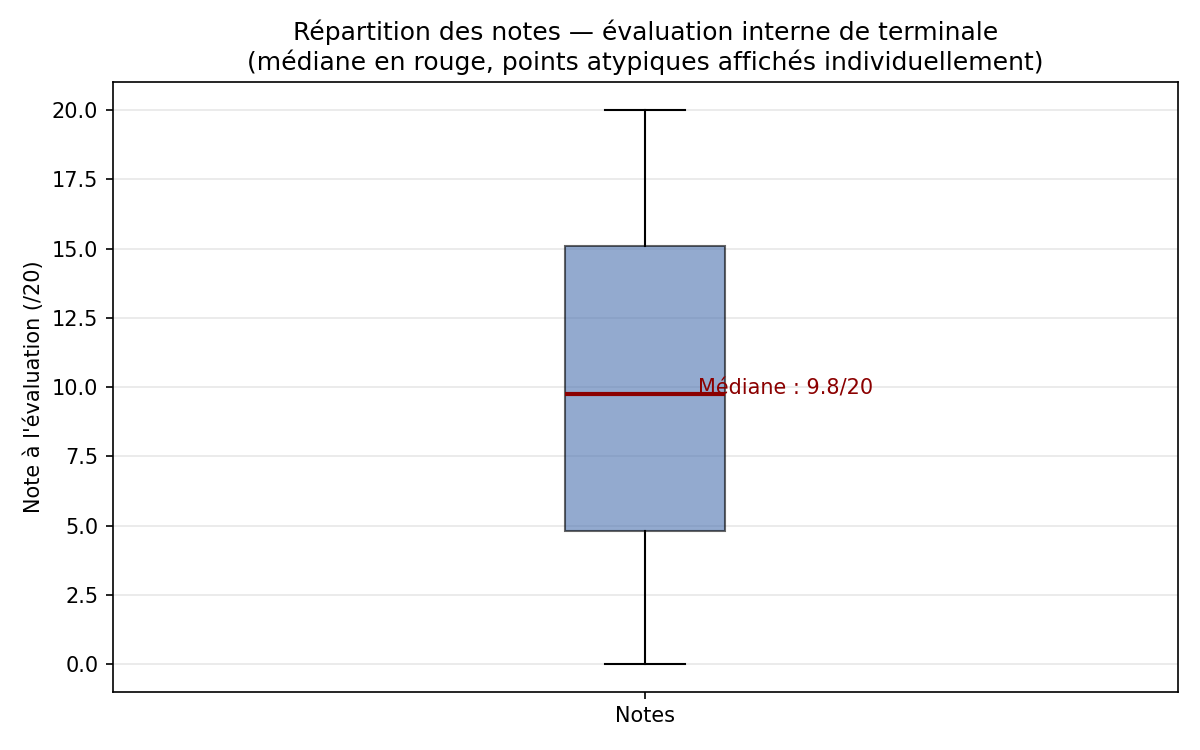
\includegraphics[width=0.75\textwidth]{figures/boxplot_notes_evaluation.png}
\caption{Boîte à moustaches des notes}
\end{figure}

\begin{figure}[H]
\centering
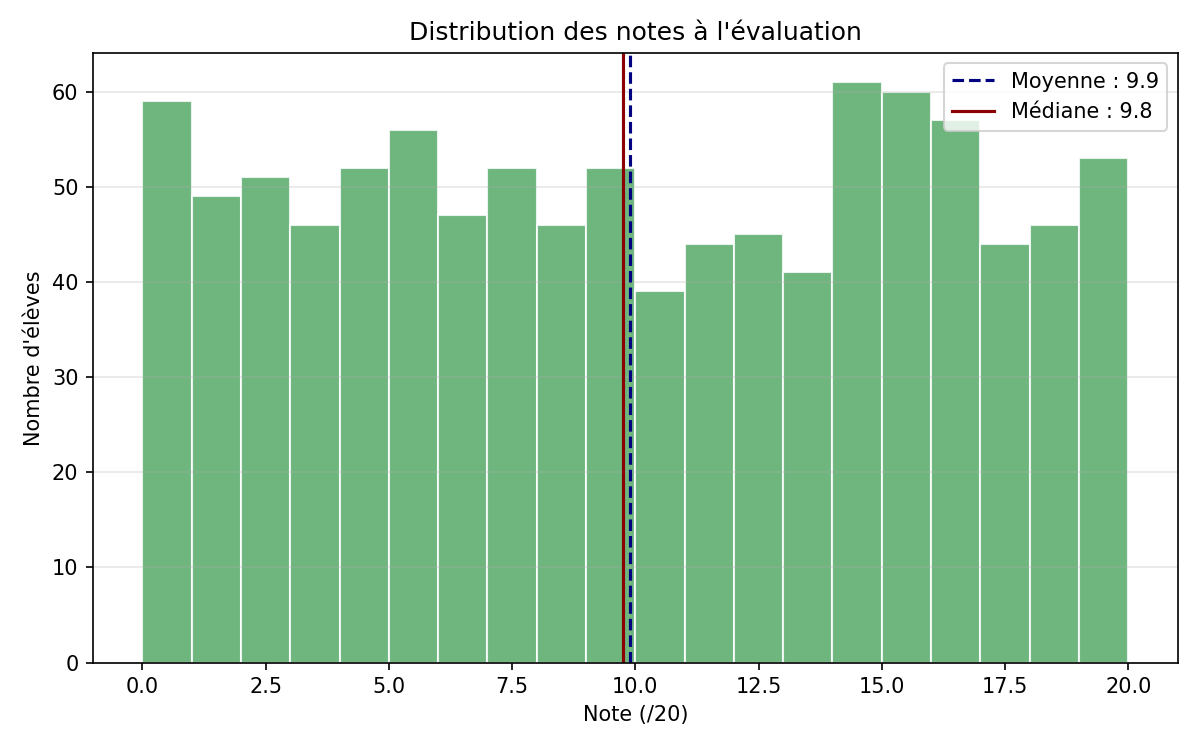
\includegraphics[width=0.75\textwidth]{figures/histogramme_notes_evaluation.png}
\caption{Histogramme des notes}
\end{figure}

\subsection{Interprétation pour le conseil pédagogique}

La médiane (9,75) est très proche de la moyenne (9,90), ce qui indique une distribution
\textbf{à peu près symétrique}. L'écart-type élevé (5,87) montre que les notes sont
étalées sur toute l'échelle 0--20, ce qui est cohérent avec le mode de génération
(tirage uniforme). Comme les bornes de Tukey ($-10,65$ et $30,55$) dépassent largement
l'intervalle possible des notes ($[0,20]$), \textbf{aucune note, même 0 ou 20, n'est
statistiquement aberrante} : ce sont des valeurs extrêmes mais plausibles dans une
distribution uniforme, pas des anomalies.

Pour un public non statisticien, il est recommandé de présenter la \textbf{boîte à
moustaches} plutôt que des tableaux de chiffres : elle montre en un coup d'œil la
médiane, l'étendue « normale » des notes et l'absence de valeurs aberrantes.

\subsection{Limites et discussion}
\begin{itemize}
\item La règle de Tukey suppose implicitement une distribution unimodale ; ici la
distribution est proche de l'uniforme, ce qui peut masquer des sous-groupes (voir Q3).
\item L'absence d'outliers statistiques ne signifie pas l'absence d'élèves en difficulté :
un élève à 2/20 n'est pas un « outlier » mais mérite un suivi pédagogique.
\end{itemize}

% ============================================================
\section{Question 2 -- Lien assiduité/note et prédiction}
% ============================================================

\subsection{Question posée}
\textit{« Le résultat est-il fortement lié à l'assiduité ? Peut-on anticiper la note des
élèves n'ayant pas encore passé l'évaluation ? À partir de quel point l'anticipation
devient-elle trop incertaine ? »}

\subsection{Volet 1 -- Vérifier le lien}

\subsubsection{Notions mobilisées}
On mesure la force du lien entre deux variables quantitatives avec les
\textbf{coefficients de corrélation de Pearson et de Spearman}, et la
\textbf{covariance}.

\begin{lstlisting}
pearson  = df["Assiduite"].corr(df["Notes"], method="pearson")
spearman = df["Assiduite"].corr(df["Notes"], method="spearman")
covariance = np.cov(df["Assiduite"], df["Notes"])[0, 1]
\end{lstlisting}

\begin{table}[H]
\centering
\begin{tabular}{|l|r|l|}
\hline
Indicateur & Valeur & Interprétation \\
\hline
Pearson (r) & 0,986 & Lien linéaire très fort \\
Spearman ($\rho$) & 0,986 & Lien monotone très fort, robuste aux outliers \\
Covariance & 169,68 & Forte co-variation \\
\hline
\end{tabular}
\caption{Indicateurs bivariés (données recalculées, graine 1292)}
\end{table}

\begin{figure}[H]
\centering
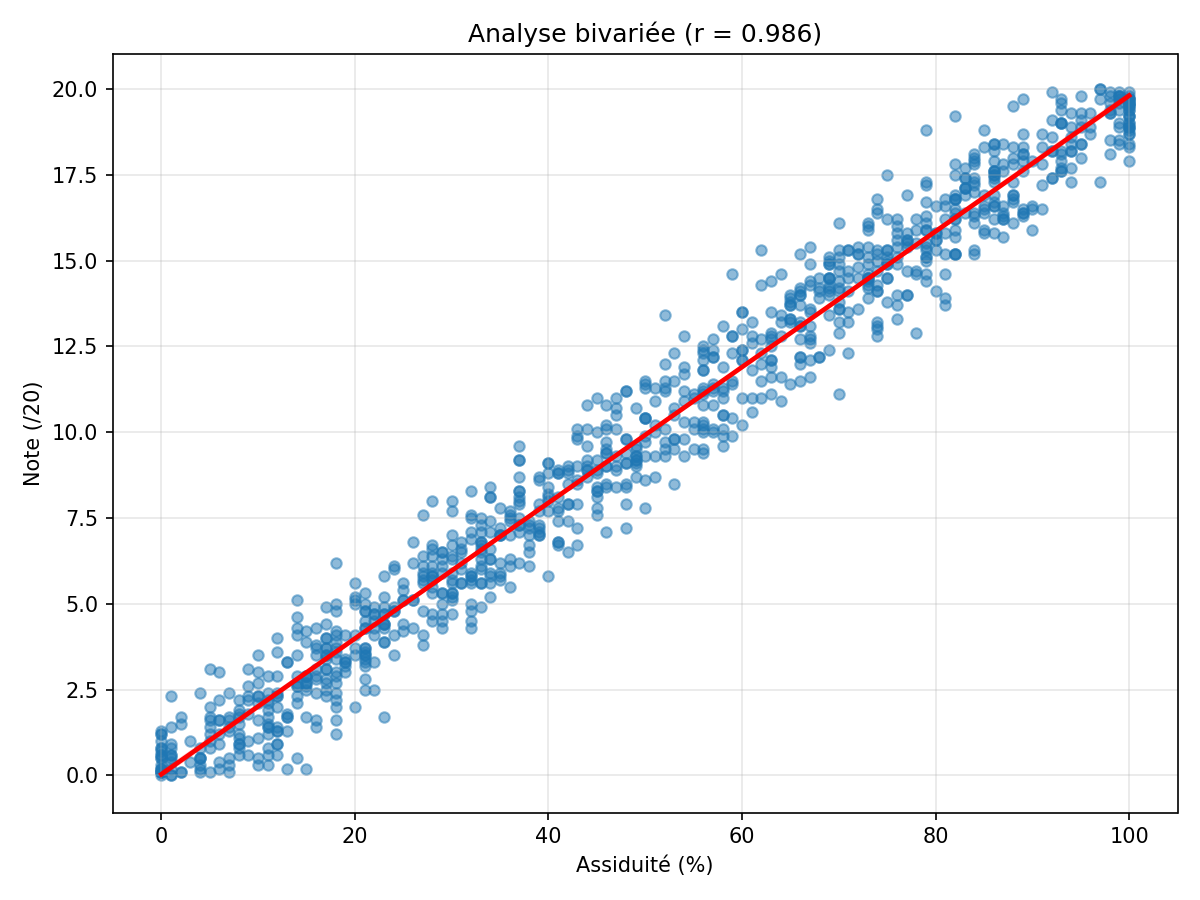
\includegraphics[width=0.6\textwidth]{figures/nuage_points_assiduite_notes.png}
\caption{Nuage de points Assiduité vs Notes}
\end{figure}

Le nuage de points confirme visuellement une relation \textbf{quasi linéaire} : les
points s'alignent sur une droite croissante, sans courbure marquée.

\subsection{Volet 2 -- Régression linéaire}

Conformément au sujet du TP (Section~5), nous modélisons la relation par une
\textbf{seule régression linéaire} : prédire \texttt{Notes} à partir de \texttt{Assiduité}.

\textbf{Pourquoi ce modèle ?}
\begin{enumerate}
\item La génération des données impose $Y \approx 5X + \varepsilon$ : structure linéaire.
\item Pearson ($r=0,986$) et Spearman ($\rho=0,986$) confirment un lien linéaire fort.
\item L'équation \texttt{Notes = a $\times$ Assiduité + b} est lisible pour le proviseur
(« +10 points d'assiduité $\Rightarrow$ environ +2 points de note »).
\end{enumerate}

\begin{lstlisting}
X_train, X_test, y_train, y_test = train_test_split(
    X, y, test_size=0.2, random_state=42)   # 800 / 200 eleves

modele = LinearRegression()
modele.fit(X_train, y_train)
y_pred = modele.predict(X_test)
\end{lstlisting}

\subsubsection{Résultats sur le jeu de test ($n=200$)}

\begin{table}[H]
\centering
\begin{tabular}{|l|r|r|r|}
\hline
Modèle & RMSE (pts) & MAE (pts) & $R^2$ \\
\hline
Régression linéaire & 1,021 & 0,835 & 0,969 \\
\hline
\end{tabular}
\caption{Performance de la régression linéaire (graine 1292)}
\end{table}

\subsubsection{Équation de la droite de régression}

\begin{equation}
\text{Notes} \approx 0{,}198 \times \text{Assiduité} + 0{,}015
\end{equation}

\textit{Interprétation : +10 points d'assiduité $\Rightarrow$ environ +2 points de note.}

\begin{figure}[H]
\centering
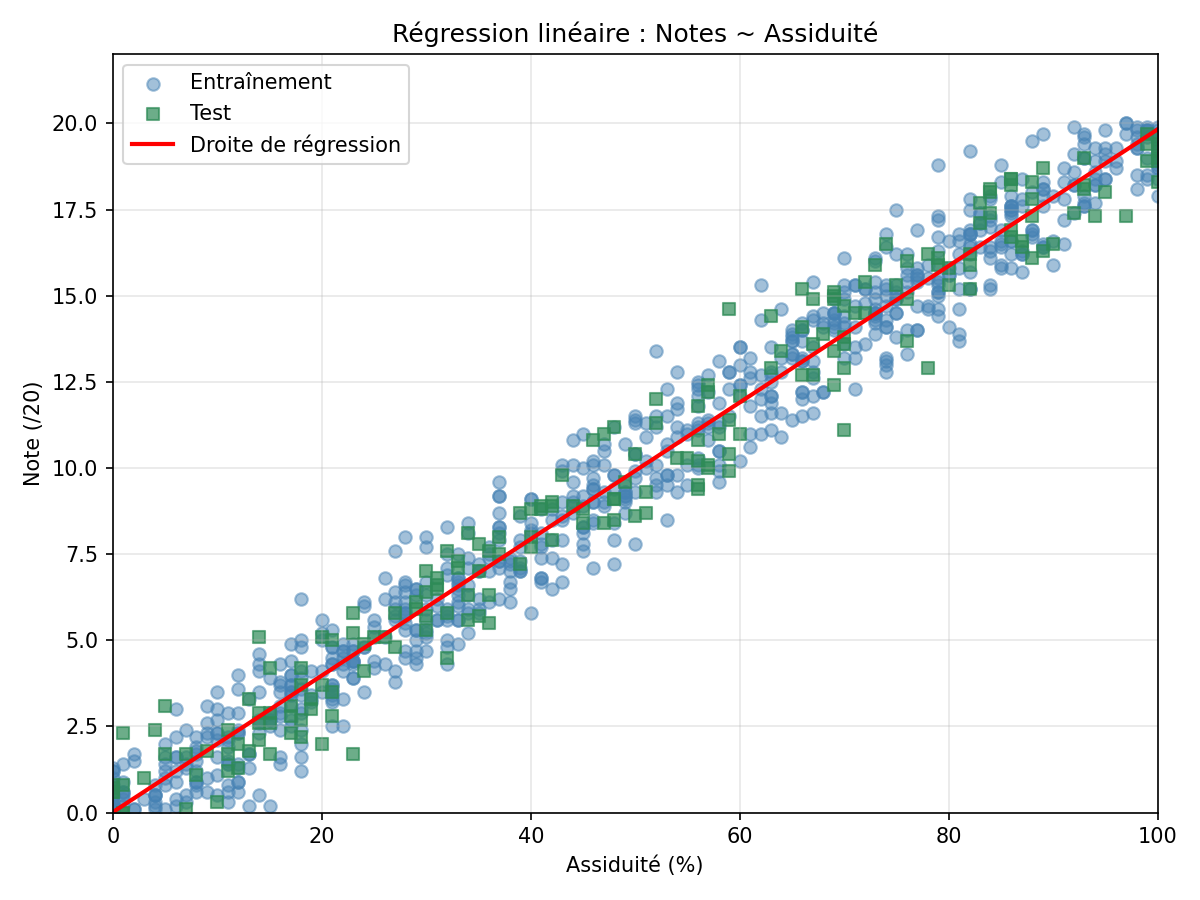
\includegraphics[width=0.65\textwidth]{figures/regression_lineaire_notes_assiduite.png}
\caption{Régression linéaire : droite de prédiction sur le jeu de test}
\end{figure}

\subsection{Seuil d'incertitude acceptable}

\textbf{Critère retenu :} une anticipation est jugée trop incertaine si la RMSE dépasse
\textbf{2 points sur 20} (10\% de la note maximale), seuil au-delà duquel l'erreur devient
trop grande pour fonder une décision individuelle.

\begin{table}[H]
\centering
\begin{tabular}{|l|r|l|}
\hline
Situation & RMSE & Décision \\
\hline
Nos données & 1,02 pt & Anticipation utilisable, avec prudence \\
Seuil limite & 2,0 pts & Au-delà, ne pas fonder une décision seule \\
\hline
\end{tabular}
\end{table}

\subsection{Limites et discussion}
\begin{itemize}
\item La relation testée ici est \textbf{univoque et synthétique} : dans un
établissement réel, l'assiduité seule n'explique jamais 97\% de la variance des notes ;
d'autres facteurs (méthode de travail, soutien familial, matière) interviennent.
\item Le modèle prédit une \textbf{note moyenne probable}, pas une certitude
individuelle : deux élèves à la même assiduité peuvent avoir des notes différentes
(le bruit gaussien du modèle de génération le montre).
\item Extrapoler en dehors de la plage observée (assiduité proche de 0\% ou de 100\%)
est risqué, la régression linéaire n'étant fiable que dans l'intervalle des données
d'entraînement.
\end{itemize}

% ============================================================
\section{Question 3 -- Profils d'élèves (clustering)}
% ============================================================

\subsection{Question posée}
\textit{« Indépendamment de l'orientation déjà recommandée, mes données font-elles
apparaître des groupes d'élèves aux profils proches ? Combien de profils distincts, et
comment les décrire ? »}

\subsection{Pourquoi l'apprentissage \emph{non supervisé} et pas du supervisé ?}

C'est un point de méthode important, qu'il faut justifier explicitement :

\begin{itemize}
\item L'apprentissage \textbf{supervisé} exige une \textbf{variable cible connue} que
l'on cherche à prédire (ex. : Q2 prédit \texttt{Notes}, Q4 prédira \texttt{target}). Or,
la question 3 ne demande \textbf{pas} de prédire l'orientation : elle demande de
découvrir des \textbf{regroupements naturels} d'élèves, sans utiliser cette étiquette,
justement pour voir si les données \emph{elles-mêmes} suggèrent une structure, avant
toute décision.
\item Utiliser \texttt{target} pour construire les groupes reviendrait à
\textbf{recopier une décision déjà prise} par le conseil de classe, ce qui ne répond pas
à la question posée (« indépendamment de l'orientation déjà recommandée »).
\item Il n'existe \textbf{aucune étiquette « profil »} dans les données : les profils
(fragile, intermédiaire, solide) ne sont pas des catégories prédéfinies mais des
regroupements à \textbf{découvrir}. C'est exactement la définition de l'apprentissage
non supervisé.
\item Le \textbf{K-Means} est retenu car les deux variables (\texttt{Notes},
\texttt{Assiduité}) sont quantitatives, les groupes attendus sont de forme
approximativement convexe (visibles sur le nuage de points de la Q2), et K-Means est
simple à interpréter pour un public non statisticien (un centroïde = un profil moyen).
\end{itemize}

\begin{lstlisting}
features = df[["Notes", "Assiduite"]]
X_scaled = StandardScaler().fit_transform(features)  # indispensable
kmeans = KMeans(n_clusters=3, random_state=42, n_init=10)
df["cluster"] = kmeans.fit_predict(X_scaled)
\end{lstlisting}

La standardisation est indispensable : sans elle, l'assiduité (échelle 0--100)
dominerait le calcul des distances et écraserait la contribution des notes
(échelle 0--20).

\subsection{Choix du nombre de clusters K}

\begin{figure}[H]
\centering
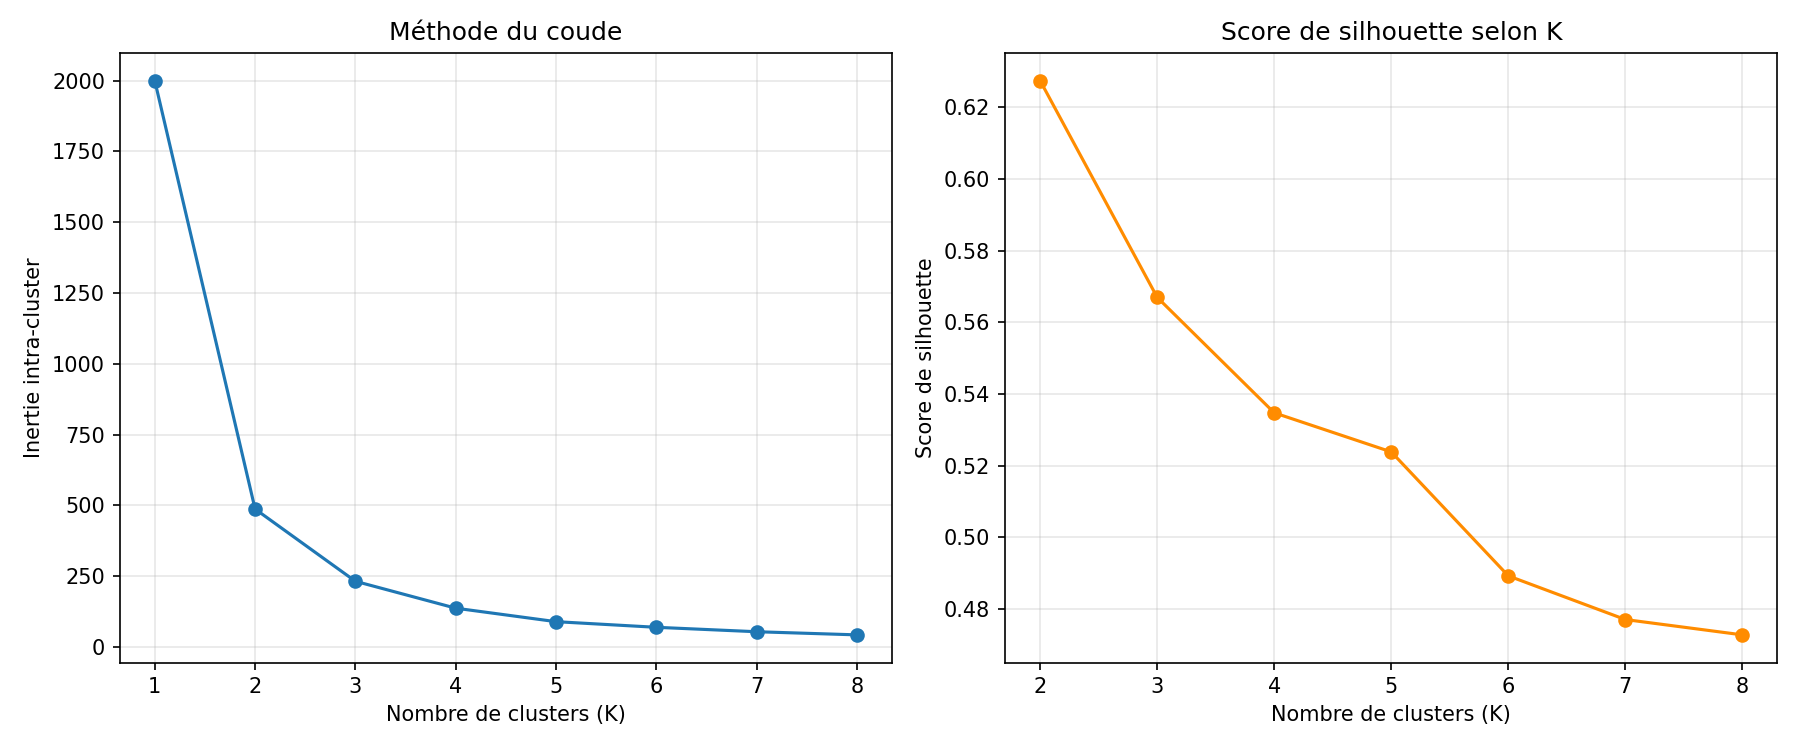
\includegraphics[width=0.85\textwidth]{figures/graphique_choix_nombre_clusters.png}
\caption{Méthode du coude (inertie) et score de silhouette}
\end{figure}

\begin{table}[H]
\centering
\begin{tabular}{|c|r|r|}
\hline
K & Inertie & Silhouette \\
\hline
2 & 487,4 & \textbf{0,627} \\
3 & 231,8 & 0,567 \\
4 & 137,2 & 0,534 \\
5 & 89,3 & 0,524 \\
\hline
\end{tabular}
\caption{Résultats recalculés (graine 1292)}
\end{table}

\textbf{Discussion honnête du choix de K :} le score de silhouette est en réalité
\textbf{maximal pour K=2} (0,627), ce qui indiquerait mathématiquement que 2 groupes
séparent le mieux les données (probablement une simple coupure « faible / forte
performance »). Nous retenons néanmoins \textbf{K=3}, pour deux raisons : (1) la baisse
d'inertie entre K=2 et K=3 reste très importante (487 $\to$ 232, soit $-52\%$), signe
qu'un découpage plus fin capture une structure réelle et pas seulement du bruit ; (2) sur
le plan \textbf{pédagogique}, 3 groupes (fragile / intermédiaire / solide) sont plus
actionnables pour le conseil pédagogique qu'une simple dichotomie « en difficulté / pas
en difficulté ». Ce choix est un compromis assumé entre optimalité statistique stricte et
utilité opérationnelle -- limite qu'il convient de signaler clairement au proviseur.

\subsection{Résultats -- 3 profils}

\begin{table}[H]
\centering
\begin{tabular}{|c|r|r|r|l|}
\hline
Cluster & Note moy. (/20) & Assiduité moy. (\%) & Effectif & Profil \\
\hline
0 & 16,4 & 82,2 & 365 & Solide \\
1 & 3,1 & 16,1 & 327 & Fragile \\
2 & 9,4 & 47,6 & 308 & Intermédiaire \\
\hline
\end{tabular}
\caption{Profils identifiés (données recalculées, graine 1292)}
\end{table}

\begin{figure}[H]
\centering
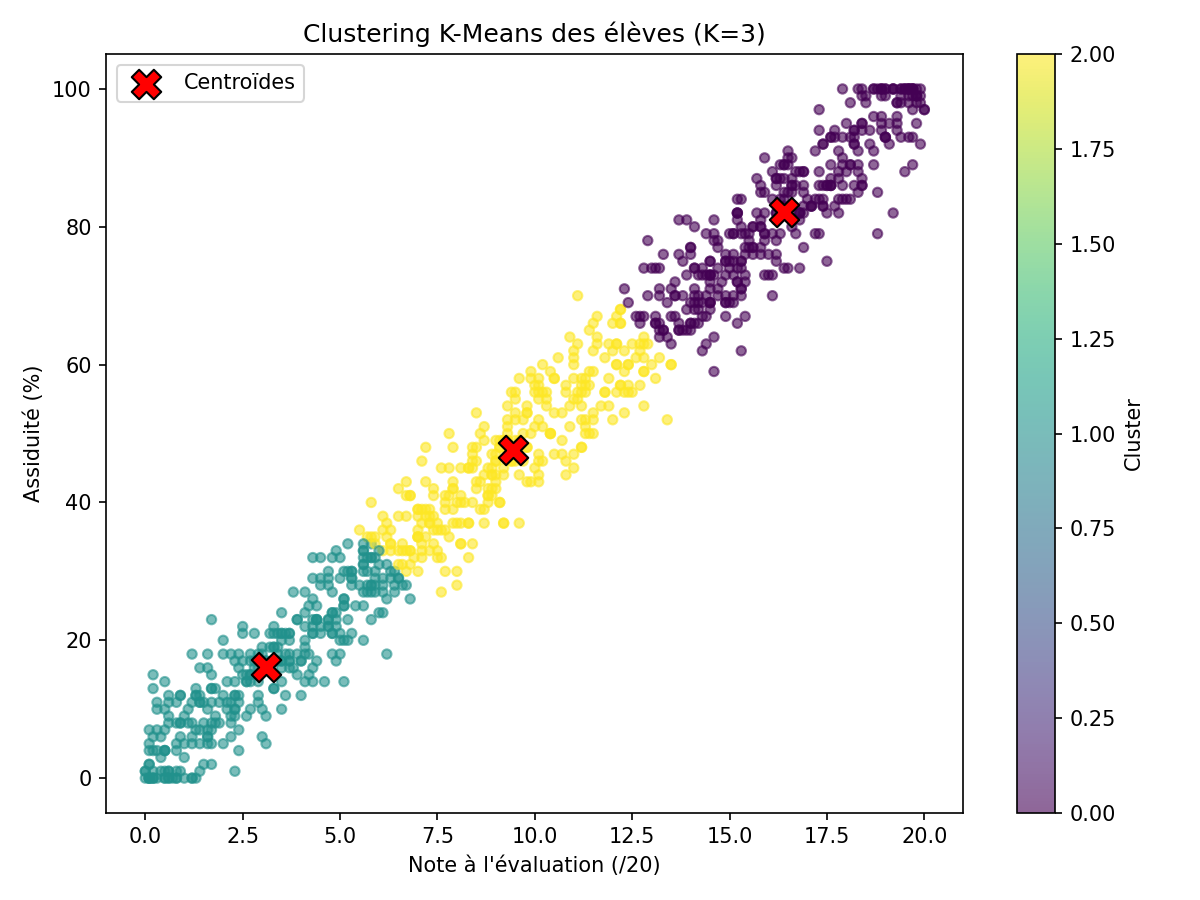
\includegraphics[width=0.7\textwidth]{figures/visualisation_clusters_eleves.png}
\caption{Visualisation des 3 clusters (les croix rouges sont les centroïdes)}
\end{figure}

\begin{itemize}
\item \textbf{Profil fragile} (327 élèves, 32,7\%) : note et assiduité très basses
\item \textbf{Profil intermédiaire} (308 élèves, 30,8\%) : résultats moyens
\item \textbf{Profil solide} (365 élèves, 36,5\%) : bonne assiduité et bons résultats
\end{itemize}

\subsection{Limites et discussion}
\begin{itemize}
\item Le clustering \textbf{décrit} des profils de performance, il ne
\textbf{prescrit} pas une filière : la correspondance profil $\leftrightarrow$
orientation n'est qu'une lecture a posteriori, non garantie.
\item Le choix K=3 reste, comme discuté ci-dessus, un compromis et non un optimum
statistique strict (K=2 obtient une meilleure silhouette).
\item K-Means suppose des clusters de forme sphérique dans l'espace standardisé ; une
structure plus complexe (non convexe) serait mal capturée par cette méthode.
\end{itemize}

% ============================================================
\section{Question 4 -- Suggestion automatique d'orientation}
% ============================================================

\subsection{Question posée}
\textit{« Pour les prochaines années, j'aimerais qu'un système puisse suggérer
automatiquement une orientation (scientifique/littéraire) pour un nouvel élève, à partir
de ses deux mesures, avant la délibération du conseil de classe. Est-ce raisonnable ?
Quelle confiance, quel risque pédagogique ? »}

\subsection{Pourquoi l'apprentissage \emph{supervisé} ici (contraste avec Q3)}

Contrairement à la question 3, on dispose ici d'une \textbf{étiquette cible connue et
exploitable} : \texttt{target} (l'orientation déjà recommandée par le conseil de classe
pour les élèves passés). L'objectif est explicitement de \textbf{prédire cette
étiquette} pour de nouveaux élèves : c'est la définition même d'un problème
d'apprentissage supervisé, ici de \textbf{classification binaire} (et non de régression,
car la cible est catégorielle : scientifique/littéraire).

\subsection{Modèles comparés}

Trois classifieurs sont comparés : la \textbf{régression logistique} (interprétable,
donne une probabilité), un \textbf{arbre de décision} (règles lisibles par un non
statisticien) et \textbf{KNN} (référence de proximité).

\begin{lstlisting}
X_train, X_test, y_train, y_test = train_test_split(
    X, y, test_size=0.2, random_state=42, stratify=y)

log_reg = LogisticRegression().fit(X_train_scaled, y_train)
arbre   = DecisionTreeClassifier(max_depth=4, random_state=42).fit(X_train, y_train)
knn     = KNeighborsClassifier(n_neighbors=5).fit(X_train_scaled, y_train)
\end{lstlisting}

\subsection{Résultats}

\begin{table}[H]
\centering
\begin{tabular}{|l|r|r|r|r|r|}
\hline
Modèle & Accuracy & Précision & Rappel & F1 & AUC \\
\hline
Arbre de décision & \textbf{1,000} & 1,000 & 1,000 & \textbf{1,000} & 1,000 \\
KNN (k=5) & 0,990 & 1,000 & 0,980 & 0,990 & 1,000 \\
Régression logistique & 0,990 & 1,000 & 0,980 & 0,990 & \textbf{1,000} \\
\hline
\end{tabular}
\caption{Comparaison des 3 classifieurs (jeu de test, n=200, graine 1292)}
\end{table}

\begin{figure}[H]
\centering
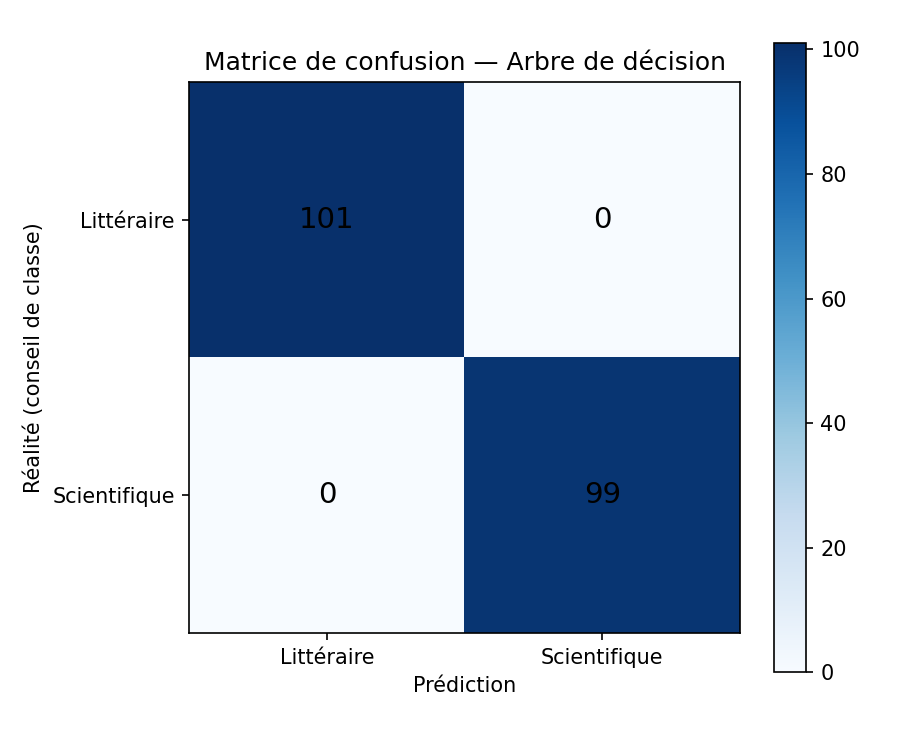
\includegraphics[width=0.55\textwidth]{figures/matrice_confusion_q4.png}
\caption{Matrice de confusion -- Arbre de décision (101 vrais négatifs, 99 vrais positifs, 0 erreur sur 200)}
\end{figure}

\begin{figure}[H]
\centering
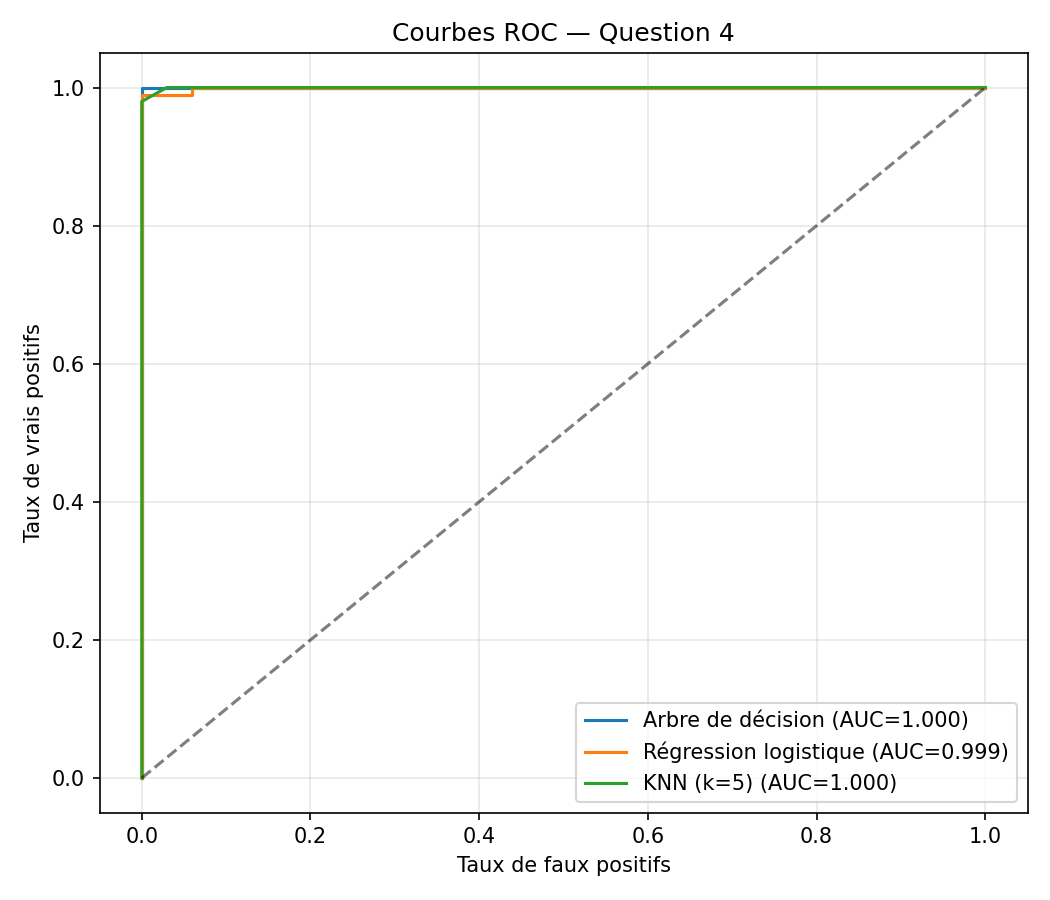
\includegraphics[width=0.55\textwidth]{figures/courbe_roc_q4.png}
\caption{Courbes ROC des 3 modèles}
\end{figure}

Validation croisée (5 blocs, régression logistique) : F1 $= 0{,}989 \pm 0{,}010$,
confirmant que la performance n'est pas due au hasard du découpage train/test.

\subsection{Est-ce raisonnable ? Quelle confiance et quel risque ?}

\textbf{Les scores sont excellents (99\% de précision, AUC proche de 1)}, mais il faut
immédiatement en relativiser la portée pour le proviseur :

\begin{enumerate}
\item \textbf{Ces performances quasi parfaites tiennent à la construction même du jeu de
données} : dans nos données synthétiques, \texttt{target} a été défini comme un simple
seuil sur l'assiduité (\texttt{target = 1 si Assiduité} $\geq$ \texttt{50\%}). Le modèle
n'a donc, pour l'essentiel, qu'à retrouver ce seuil -- ce qui est un problème beaucoup
plus facile qu'une vraie décision d'orientation.
\item \textbf{Dans la réalité}, une décision d'orientation du conseil de classe repose
sur bien plus que deux variables (bulletins complets, avis des professeurs de plusieurs
matières, projet de l'élève, entretiens). Un modèle entraîné sur seulement 2 variables
sous-estimera cette richesse et \textbf{ne doit pas être considéré comme fiable au même
niveau} sur des données réelles.
\item \textbf{Risque d'automatisation excessive (« automation bias »)} : un score
affiché à 99\% peut donner une fausse impression de certitude absolue et pousser à ne
plus remettre en cause la suggestion automatique, y compris dans les cas limites (proche
de la frontière de décision) où l'erreur est justement la plus probable.
\item \textbf{Risque d'effet de raccourci} : la frontière de décision apprise
(ci-dessous) est quasiment une droite correspondant au seuil d'assiduité utilisé pour
générer les données -- un système réel pourrait de la même façon apprendre une règle
biaisée si les décisions historiques du conseil de classe reflètent elles-mêmes des
biais (origine sociale, établissement d'origine, etc.), que le modèle reproduirait
alors aveuglément.
\end{enumerate}

\begin{figure}[H]
\centering
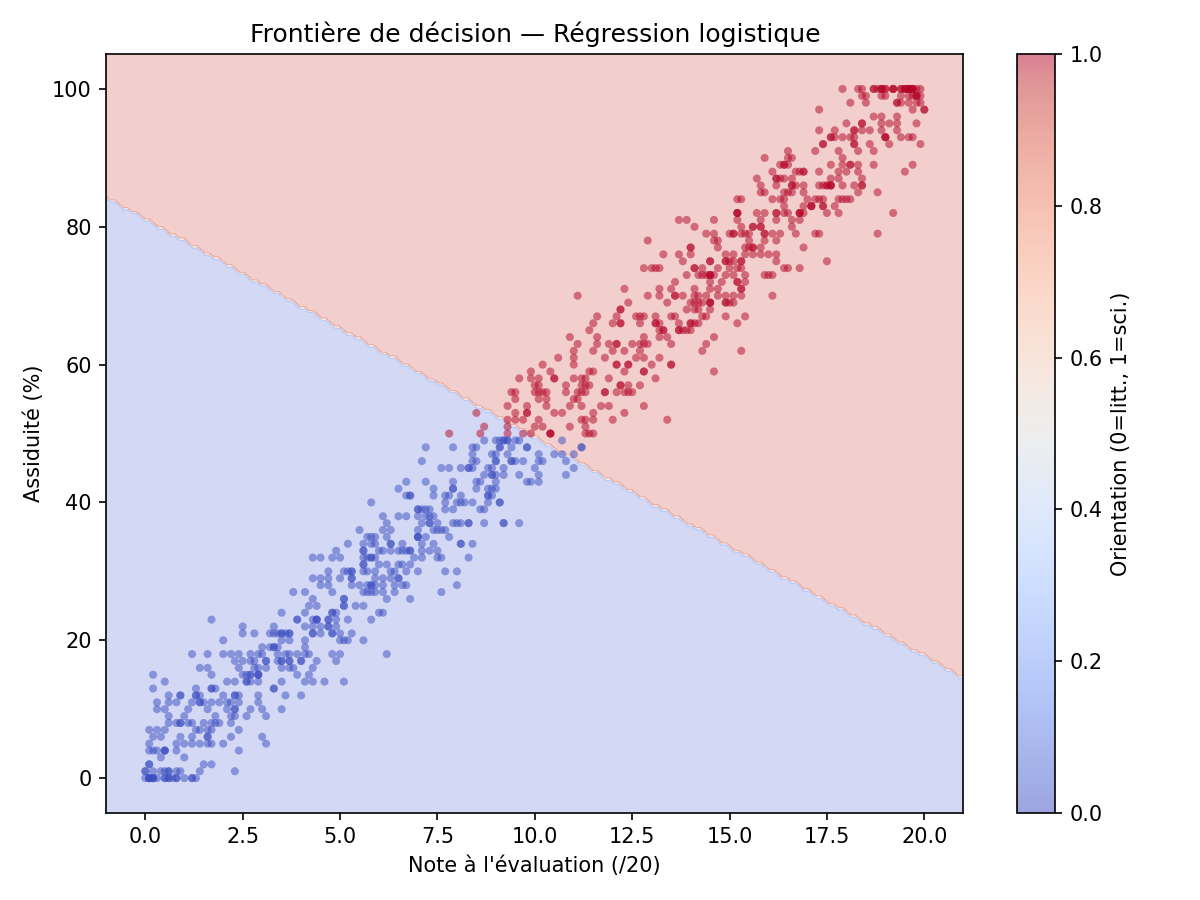
\includegraphics[width=0.65\textwidth]{figures/frontiere_decision_q4.png}
\caption{Frontière de décision apprise par la régression logistique}
\end{figure}

\subsection{Recommandation}

\textbf{Oui, un système de suggestion automatique est techniquement réalisable}, mais il
doit rester un \textbf{outil d'aide à la décision, pas un système de décision} :
\begin{itemize}
\item afficher une \textbf{probabilité} plutôt qu'une décision binaire, pour laisser
apparaître les cas incertains (proches de 50\%) ;
\item réserver l'intervention humaine systématique pour les cas où la probabilité est
proche de la frontière de décision ;
\item ne jamais utiliser le système \textbf{seul}, mais toujours en complément de
l'avis du conseil de classe, en particulier tant que le modèle n'est validé que sur des
données synthétiques à seulement 2 variables.
\end{itemize}

% ============================================================
\section{Synthèse pour le proviseur}
% ============================================================

\begin{table}[H]
\centering
\begin{tabular}{|p{2.5cm}|p{11cm}|}
\hline
\textbf{Question} & \textbf{Réponse synthétique} \\
\hline
Q1 -- Répartition &
Les notes se répartissent de façon relativement uniforme entre 0 et 20 (médiane 9,75/20).
Aucun élève n'est statistiquement atypique selon la règle de Tukey. La boîte à
moustaches est le support le plus lisible pour le conseil pédagogique. \\
\hline
Q2 -- Lien et prédiction &
Le lien assiduité/note est confirmé (r = 0,986). La régression linéaire permet d'estimer
une note probable avec une erreur moyenne d'environ 1 point sur 20 (RMSE = 1,02). En dessous du seuil
de 2 points, l'anticipation est utilisable comme indication, jamais comme substitut à
l'évaluation réelle. \\
\hline
Q3 -- Profils &
3 profils d'élèves émergent naturellement (sans utiliser l'orientation) : fragile
(32,7\%), intermédiaire (30,8\%), solide (36,5\%). Ces profils décrivent des situations
scolaires et peuvent guider un accompagnement différencié, sans se substituer aux
décisions d'orientation déjà prises. \\
\hline
Q4 -- Suggestion automatique &
Un modèle de classification atteint une précision très élevée (100\% pour l'arbre,
99\% pour les autres) sur nos données,
mais ce résultat est en grande partie un artefact de la construction du jeu de données.
Un tel système est envisageable comme \textbf{aide} à la décision (probabilité affichée,
vigilance sur les cas proches de la frontière), mais présente un risque réel
d'automatisation excessive s'il est utilisé seul, sans validation sur des données
réelles et sans les autres éléments d'appréciation du conseil de classe. \\
\hline
\end{tabular}
\caption{Synthèse des réponses aux quatre questions du proviseur}
\end{table}

\subsection{Recommandations générales}
\begin{enumerate}
\item Ne jamais automatiser entièrement les décisions d'orientation : les modèles
estiment et décrivent, ils ne remplacent pas le conseil de classe.
\item Croiser systématiquement les sources : notes, assiduité, contrôles continus,
entretiens.
\item Utiliser les visualisations (boîte à moustaches, nuage de points, carte des
clusters, courbe ROC) comme supports de discussion en réunion pédagogique plutôt que des
tableaux de chiffres bruts.
\item Garantir la reproductibilité : l'ensemble des analyses est rejouable via
\texttt{python main.py}, avec la graine corrigée 1292.
\end{enumerate}

\end{document}
